\subsection[]{Dimostrare l’espressione
\[
	\frac{dt}{dt'}=1-\hat{n}\bs{\beta}
.\] 
dove t e t’ sono il tempo di osservazione ed il tempo ‘ritardato’, rispettivamente.}
\label{sec:3.a.1}
Si prenda una carica che si muove con la legge oraria $\bs{s}\left( t \right) $ e velocità $\bs{\beta}$, sfruttando la definizione di tempo ritardato: \[
	t=t_{\text{rit}} + \left| \bs{r}- \bs{s}\left( t_{\text{rit}} \right)  \right|/c 
.\]
Possiamo differenziare: \[
	\frac{\mbox{d} t}{\mbox{d} t_{\text{rit}}} = 1- \frac{\bs{r}-\bs{s}\left( t_{\text{rit}} \right) \cdot \frac{\mbox{d} \bs{s}\left( t_{\text{rit}} \right) }{\mbox{d} t_{\text{rit}}} }{\left| \bs{r}-\bs{s}\left( t_{\text{rit}} \right)  \right|c }=\left.1-\hat{n}\cdot \bs{\beta}\right|_{\text{rit}}
.\] 
\subsection[]{Date le definizioni ‘standard’ delle variabili $\hat{n}, \bs{\beta}, \bs{R}, \bs{r}, \bs{r}', t, t'$ , dimostrare le seguenti relazioni:
} \label{sec:3.b.2}
\begin{align*}
&1) \ \frac{\mbox{d} \bs{R}}{\mbox{d} t'} = -\bs{\beta}c 					&2)& \ \frac{\mbox{d}R}{\mbox{d}t'}=-\hat{n}\cdot\bs{\beta}c\\
& & &\\
&3) \ \frac{\mbox{d}\left(\bs{R}\cdot\bs{\beta}\right)}{\mbox{d}t'}=-\beta c+\bs{R}\cdot\bs{\beta}	&4)& \ \nabla\bs{R}=\frac{\hat{n}}{\left(1-\hat{n}\bs{\beta}\right)}\\
& & &\\
&5) \ \nabla t' = \frac{-\hat{n}/c}{1-\hat{n}\bs{\beta}}
.\end{align*}
Si ha che $\bs{r}$ e $t$ sono il punto e l'istante in cui si osservano i campi , $\bs{r}'$ la posizione delle sorgenti. $t'$ è il tempo ritardato definito da : \[
	c\left( t-t' \right) =\left| \bs{r}- \bs{r}'\left( t' \right)  \right| 
.\] 
Si ha inoltre che \[
	\bs{R}= \bs{r}-\bs{r}'\left( t' \right) 
.\]
Mentre $\hat{n} = \bs{R} /R$ e $\bs{\beta}=\dot{\bs{r}}' /c$. Possiamo inoltre derivare $\bs{R}$ rispetto al tempo ritardato per ottenere una delle relazioni: \[
	\frac{\mbox{d} \bs{R}}{\mbox{d} t'} = -\dot{\bs{r}}'=-\bs{\beta}c
.\] 
Facciamo quindi lo stesso con $R$ : \[
	\frac{\mbox{d} R}{\mbox{d} t'} = \frac{\mbox{d} \left| \bs{r}-\bs{r}' \right| }{\mbox{d} t'} = 
	\frac{\bs{R}}{R}\cdot \frac{\mbox{d} \bs{R}}{\mbox{d} t'}= - \hat{n}\cdot \bs{\beta}c
.\] 
E con il prodotto $\bs{R}\cdot \bs{\beta}$ : \[
	\frac{\mbox{d} \left( \bs{R}\cdot \bs{\beta} \right) }{\mbox{d} t'} = \bs{\beta}\cdot \frac{\mbox{d} \bs{R}}{\mbox{d} t'} + \bs{R}\frac{\mbox{d} \bs{\beta}}{\mbox{d} t'} = -\beta^2c + \bs{R}\cdot \dot{\bs{\beta}} 	
.\]
Dalla definizione di tempo ritardato si ha una utile relazione tra $\nabla t'$ e $\nabla R$ : \[
	-c\nabla t' = \nabla R 
.\] 
È necessario calcolare solo $\nabla t'$ per avere anche l'altra quantità:
\begin{align*}
	-c\nabla t' &= \nabla \left| \bs{r}-\bs{r}'\left( t' \right)  \right| =\\
		    &= \hat{x}_{i} \frac{\partial }{\partial x_{i} } \sqrt{\sum_{j=1}^{3} \left( r_{j}-r'_{j}\left( t' \right)  \right)^2 }=\\
		    &= \frac{\hat{x}_{i}}{2R} \frac{\partial }{\partial x_{i}} \sum_{j=1}^{3} \left( r_{j}-r'_{j}\left( t' \right)  \right) ^2 = \\
		    &= \frac{\hat{x}_{i}}{R} \sum_{j=1}^{3} \left( r_{j}-r'_{j}\left( t' \right)  \right)
		    \left( \delta_{ij}-c \beta_{j}\left( t' \right) \frac{\partial t'}{\partial x_{i}}  \right) =\\
		    &= \hat{n}- c \hat{n}\cdot \bs{\beta} \nabla t' 
.\end{align*}
Se ne conclude che : \[
	\nabla t'=-\frac{\hat{n} /c}{1-\hat{n}\cdot \bs{\beta}}
.\] 

\subsection[]{Calcolare la distribuzione in potenza in funzione dell’angolo di emissione per una carica accelerata in moto non relativistico.}
\label{sec:3.b.3}
Si parte dal campo generato da una carica in moto :
\[
	\bs{E}\left( \bs{x},t \right) = q \left[ \frac{\hat{n}-\bs{\beta}}{\gamma^2\left( 1-\hat{n}\cdot \bs{\beta} \right)^3 R^2 } \right]_{\text{rit}}+
	\frac{q}{c} \left[ \frac{\hat{n}\wedge \left[ \left( \hat{n}-\bs{\beta} \right) \wedge \dot{\bs{\beta}}  \right] }
	{\left( 1-\hat{n}\cdot \bs{\beta} \right) R}  \right]_{\text{rit}} 
.\] \label{eq:L-W} 
Dove le quantità sono quelle definite nella domanda precedente. Si trascura adesso il campo a decrescsenza rapida e si considera solo il campo di radiazione approssimandolo al caso non relativistico:
\[
	\bs{E}_{\text{rad}}\left( \bs{x},t \right)= \frac{q}{c} \left[ \frac{\hat{n}\wedge \left[ \left( \hat{n}-\bs{\beta} \right) \wedge \dot{\bs{\beta}}  \right] }
	{\left( 1-\hat{n}\cdot \bs{\beta} \right) R}  \right]_{\text{rit}}  \approx \frac{q}{c} \left[ \frac{\hat{n}\wedge \left( \hat{n}\wedge \dot{\bs{\beta}}\right)}{R} \right]_{\text{rit}} 
.\] 
L'approssimazione si ottiene raggruppando un $\hat{n}$ al numeratore. IL vettore di Poynting quindi è:
\[
	\bs{S}= \frac{c}{4 \pi} \left| \bs{E}_{\text{rad}} \right| ^2 \hat{n}=\frac{q^2}{4\pi c^3} 
	\left| \frac{\hat{n}\wedge \left( \hat{n}\wedge  \dot{\bs{\beta}}\right)}{R} \right|^2
.\] 
Dove si è anche trascurato il termine $\bs{\beta}$ rispetto al ternine $\hat{n}$ perchè discutiamo il caso  non relativistico. Andando adesso in un sistema di riferimento in cui $\theta$ è l'angolo tra la accelerazione della particella e la direzione di osservazione si ha:
\[
	\bs{S}= \frac{q^2}{4\pi R^2 c^3}\sin^2\theta \left| \dot{\bs{v}} \right| ^2 \hat{n}
.\] 
In conclusione si trova la distribuzione angolare di potenza come:
\[
	\frac{\mbox{d} P}{\mbox{d} \Omega} = \frac{\mbox{d} P}{\mbox{d} \Sigma } \frac{\mbox{d} \Sigma}{\mbox{d} \Omega}=
	\left| \bs{S} \right| R^2 = \frac{q^2}{4\pi c^3} a^2 \sin^2\theta
.\] 

\subsection[]{Ricavare esplicitamente le leggi di trasformazione di Lorentz del campo elettrico e del campo magnetico. Discutere, in particolare, il caso in cui, in un certo sistema di riferimento inerziale, il campo magnetico è nullo e il caso in cui il campo elettrico è nullo.}
\label{sec:3.b.4}
Il modo migliore per vedere come trasformano i campi è vedere come trasforma il tensore dei campi. Per semplicità scegliamo un boost lungo l'asse $x$, tale tensore (antisimmetrico) trasforma come :
\[
	F'^{\alpha\beta}= \Lambda^{\mu}_{\alpha} \Lambda^{\nu}_{\beta} F^{\alpha\beta}
.\] 
Si può adesso procedere in due modi: calcolo indiciale o calcolo matriciale, si tratta qua la prima strada.Per completezza si aggiunge solo che brutalmente il conto con le matrici sarebbe:\[
	F'=\Lambda F \Lambda^{t}
.\] 
Dove $\Lambda$ è:
\[
	\Lambda = 
	\left( 
	\begin{array}{cccc}
		\gamma & -\beta\gamma & 0 & 0 \\   
		-\beta\gamma & \gamma & 0 & 0 \\
		0 & 0 & 1 & 0 \\
		0 & 0 & 0 & 1 \\
	\end{array}
	\right) 
.\]
Mentre $F$ è:
\[
	F = 
	\left( 
	\begin{array}{c|ccc}
		0 & -E_{x} & -E_{y} & -E_{z} \\   
		\hline
		E_{x} & 0 & -B_{z} & B_{y} \\
		E_{y} & B_{z} & 0 & -B_{x} \\
		E_{z} & -B_{y} & B_{x} & 0 \\
	\end{array}
	\right) 
.\] 
Se non vogliamo morire di conti bisogna essere astuti. Calcoliamo alcune componenti del tensore trasformato: \[
	F'^{0i}=\Lambda^{0}_{\alpha}\Lambda^{i}_{\beta}F^{\alpha\beta}
.\] 
Quindi per la prima riga si ha : 
\begin{align*}
	F'^{01}=& -E'_{x}= \Lambda^{0}_{0}\Lambda^{1}_{0}F^{00} + \Lambda^{0}_{1}\Lambda^{1}_{1}F^{01} + 
		\Lambda^{0}_{1}\Lambda^{1}_{0}F^{10} + \Lambda^{0}_{0}\Lambda^{1}_{1}F^{11}=\\
		=&\gamma\cdot \left( -\beta\gamma \right) \cdot 0 + \gamma \cdot \gamma \cdot F_{01} +
		\left( - \beta\gamma \right) \cdot \left( -\beta\gamma \right) F + 0 = \ldots = F^{01} = -E_{x}\\ 
		 & \\
	F'^{02}=&-E'_{y}= \Lambda^{0}_{0}\Lambda^2_2 F^{02} + \Lambda^0_1\Lambda^2_2 F^{22}=\\
		=&\gamma\cdot 1\cdot F^{02}+\left(-\beta\gamma\right)\cdot 1\cdot F^{12}=\gamma\left(F^{02}-\beta F^{12}\right)=-\gamma\left(E_{y}-\beta B_{z}\right)\\
		& \\
	F'^{03}=&-E'_{z}=\Lambda^{0}_{0}\Lambda^{3}_{3}F^{03}+\Lambda^{0}_{1}\Lambda^{3}_{3}F^{13}= -\gamma\left( E_{z}+\beta B_{y} \right) 
.\end{align*}
Il calcolo faticoso ha dei vantaggi: il tensore rimmarrà antisimmetrico, quindi abbiamo già scritto la prima riga e la prima colonna. Per i rimanenti 3 elementi si trova:
\begin{align*}
	F'^{12}=& -B'_{z}= -\gamma\left(B_{z} -\beta E_{y} \right)\\ 
	F'^{13}=& B'_{y}= \gamma\left( B_{y}+\beta E_{z} \right)\\ 
	F'^{23}=& -B'_{x}= -B_{x}
.\end{align*}
Quindi il tensore trasformato risulta :
\[
F'=
\left( 
\begin{array}{cccc}
	0 				&	 -E_{x} 			& 	-\gamma ( E_{y}- \beta B_{z})  	&	 -\gamma (E_{z}+\beta B_{y}) \\   
	E_{x} 				&	 0 				& 	-\gamma ( B_{z}-\beta E_{y} )  	& 	\gamma ( B_{y}+\beta E_{z} )  \\
	\gamma ( E_{y}- \beta B_{z} )  	&	 \gamma ( B_{z}-\beta E_{y} )  	&	 0 				&	 -B_{x} \\
	\gamma ( E_{z}+\beta B_{y} )  	& 	-\gamma ( B_{y}+\beta E_{z} )  	& 	B_{x} 				& 	0 \\
	\end{array}
	\right) 
.\] 
\paragraph{Sistema con campo magnetico nullo}%
Un sistema di esempio è quello solidale ad una carica, un questo caso non essendoci moto di carica si ha $\bs{B}=0$ quindi il tensore dei campi è:
\[
F'_{B=0}=
\left( 
\begin{array}{cccc}
	0 & -E_{x} & -\gamma E_{y} & -\gamma E_{z} \\   
	E_{x} & 0 & \gamma\beta E_{y} & \gamma\beta E_{z} \\
	\gamma E_{y} & -\gamma\beta E_{y} & 0 & 0 \\
	\gamma E_{z} & -\gamma\beta E_{z} & 0 & 0 \\
\end{array}
\right) 
.\]
Da cui guardando le componenti se ne deduce la relazione: $ \bs{B}'=\bs{\beta}\wedge \bs{E}' $
\paragraph{Sistema con campo elettrico nullo}%
Un buon esempio qua è un plasma che si dispone sempre in modo da annullare il campo in questione, quindi :
\[
F'_{B=0}=
\left( 
\begin{array}{cccc}
	0 & 0 & \gamma\beta B_{z} & -\gamma\beta B_{y} \\   
	0 & 0 & -\gamma B_{z} & \gamma B_{y} \\
	-\gamma\beta B_{z} & \gamma B_{z} & 0 & -B_{x} \\
	\gamma\beta B_{y} & -\gamma E_{z} & B_{x} & 0 \\
\end{array}
\right) 
.\] 
Analogamente a sorpra se ne deduce che $\bs{E}'=-\bs{\beta}\wedge \bs{B}' $

\subsection[]{Dire quali sono gli "invarianti di Lorentz" che si possono costruire con il tensore del campo elettromagnetico e ricavarne le espressioni esplicite in termini dei campi elettrico e magnetico. Ridiscutere, usando gli invarianti, il caso discusso nel punto precedente e discutere il caso in cui gli invarianti sono nulli.}
\label{sec:3.b.5}
Possiamo costruire due invarianti indipendenti:
\begin{align*}
	F_{\mu\nu}F^{\mu\nu}=&A=F_{0i}F^{0i}+F_{i 0}F^{1 0} + F_{ij}F^{ij}=\\ 
	=& E_{i}\cdot \left( -E_{i} \right)+\left( -E_{i}\right)\cdot E_{i} + \epsilon_{ijl}B_{l}\cdot \epsilon_{ijk}B_{k}=-2\left| E \right|^2 + 2\left|B\right|^2\\
	F_{\mu\nu}\tilde{F}^{\mu\nu}=&B=\ldots=-4 \bs{E}\cdot \bs{B}
.\end{align*}
Nel caso di un sistema in cui $B=0$ si ha anche $A=0$ e $B>0$ per ogni sistema inerziale. Questo significa che i due campi sono sempre ortogonali e che il campo elettrico ha modulo maggiore del campo magnetico in ogni sistema inerziale.
Nel caso di un sistema in cui $E=0$ si ha $A=0$ e $B<0$, da questo segue una discussione complementare a quella esposta sopra.

\subsection[]{Una carica elettrica Q si muove con velocità costante su una retta con velocità costante:
\begin{align*}
	 &x=Vt \\
	 &y=b \\ 
	 &z=0
.\end{align*}
Calcolare in funzione del tempo il campo elettrico ed il campo magnetico generato dalla carica nel punto O e produrre il grafico di ognuna delle 6 componenti trovate in funzione del tempo t.}
\label{sec:3.b.6}
Il calcolo del campo elettrico è stato affrontato nella \hyperref[sec:3.a.15]{Domanda 3.a.15}, per sfruttarlo aggiungiamo che in quel caso era la carica a passare per l'origine, mentre l'osservatore a distanza b. Per simmetria inverteno osservatore e carica si ottiene lo stesso risultato della domanda citata, ovvero:
\begin{align*}
	&E_x = -e \frac{\gamma vt}{\left( \gamma^2v^2t^2 + b^2 \right)^{3 /2} }\\
	&E_y = e \frac{b\gamma }{\left( \gamma^2v^2t^2 + b^2 \right)^{3 /2}}\\
	&E_z = 0
.\end{align*}
Calcoliamo quindi il campo magnetico come $\bs{B}= \bs{\beta}\wedge \bs{E}=v/c \cdot E_{y} \hat{z}$ :
\[
	B_z = e \frac{b\gamma c}{c\left( \gamma^2v^2t^2 + b^2 \right)^{3 /2}}\\
.\] 
Per avere un quadro degli andamenti basta quindi plottare i campi elettrici. Al variare di $\beta$ nel seguente plot si riporta come questi ultimi si modificano (con la convenzione che la linea si assottiglia mano a mano che $\beta$ aumenta).
\begin{figure}[H]
	\centering
	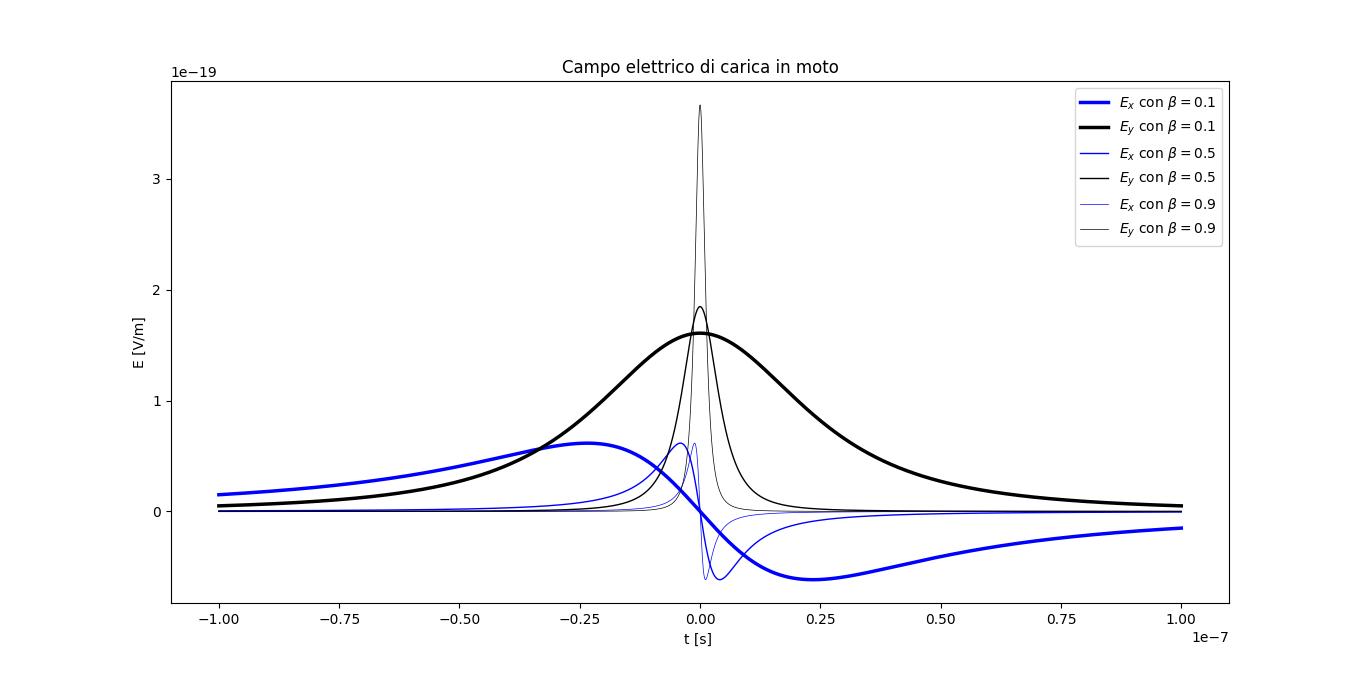
\includegraphics[width=0.8\textwidth]{immagini/carica_in_moto.png}
	\caption{Campi elettrici generati da una carica in moto}
	\label{fig:campo_carica_moto}
\end{figure}
Da notare che il campo lungo $y$ diventa sempre più stretto e piccato all'aumentare di $\beta$ (di conseguenza anche il campo magnetico).

\subsection[]{Scrivere in forma covariante l'equazione del moto di una carica in un campo elettromagnetico esterno ("quadri-forza di Lorentz").}
\label{sec:3.b.7}
Analizziamo il caso di una particella puntiforme, nel caso non relativistico avremmo: \[
	\frac{\mbox{d} \bs{p}}{\mbox{d} t} = e\left( \bs{E}+ \frac{\bs{v}}{c}\wedge \bs{B} \right) 
.\] 
È quindi ragionevole pensare che si debba sfruttare il 4-impulso $p^{\mu}=m u^{\mu}$ con $u^{\mu}=\gamma\left( c, \bs{v} \right)$, ed il tensore dei campi gia introdotto nelle domande precedenti. Per procedere si cerca una equazione della forma:
\[
	\frac{\mbox{d} p^{\mu}}{\mbox{d} \tau}= N F^{\mu\nu} u_{\nu} 
.\]
Cercando una normalizzazione ragionando sulle dimensioni: per trarre una forza dall'espressione di destra ci serve una carica a moltiplicare ed una velocità a dividere, si prova ad utilizzare $\frac{e}{c}$. Si prova quindi componente per componente:
\begin{align*}
	F^{0i}u_{i}=& -E_{i}\cdot \left( -\gamma v_{i} \right) =\gamma \bs{E}\cdot \bs{v}\\
	F^{i\alpha}u_{\alpha}=&F^{i 0}u_0+F^{ij}u_{j}=E_{i}c\gamma-\epsilon_{ijk}B_{k}\left( -\gamma v_{j} \right) =\\
	=& c\gamma\left(\bs{E}+\frac{\bs{v}}{c}\wedge \bs{B}   \right) 
.\end{align*}
Considerando il fatto che 
\[
	dt= \gamma d\tau
\]
si ha che li componenti spaziali (le seconde calcolate) danno proprio l'equazione del moto.\\
Considerando invece che $P^{\mu}=\left(\varepsilon /c, \bs{p} \right)$ si ha che la componente temporale rappresenta il teorema delle forze vive:
\[
	\frac{\mbox{d} \varepsilon}{\mbox{d} t} = e \bs{E}\cdot \bs{v}	
.\] 


\subsection[]{Dimostrare che la forza di reazione radiativa è: 
\[
	\bs{F}_{\text{rad}}=\frac{2q^2}{3c^3}\dot{\bs{a}}=z^2m_e \tau_e \dot{\bs{a}} \quad \quad \text{con } \tau_e=\frac{2r_{e}}{3c}=\left(6.2\cdot 10^{-24}\right)
.\]
Indicare inoltre il campo di applicazione di quest'ultima.
}\label{sec:3.b.8}
La dimostrazione euristica e non relativistica è stata affrontata nella \hyperref[subsec: 2.a.15]{Domanda 2.a.15} insieme ai campi di applicazione (moto periodico). 

\subsection[]{Dare la definizione del "tensore energia-impulso" del campo elettromagnetico e scrivere la sua relazione con la "densità di forza di Lorentz".}
\label{sec:3.b.9}
Il tensore energia impulso è definito come:
\[
	\Theta^{\mu\nu}=\frac{1}{4\pi}\left( F^{\mu\alpha}F^{\nu}_{\alpha}- \frac{1}{4}\eta^{\mu\nu}F^{\alpha\beta}F_{\alpha\beta} \right) 
.\] 
Dove $\eta^{\mu\nu}$ è il tensore metrico diag$\left( 1,-1,-1,-1 \right)$.\\
Per inquadrarlo meglio lo si può vedere sotto forma di matrice: 
\[
	 \Theta= 
	 \left(
		 \begin{array}{c|ccc}
			 u_{\text{em}} 	& 		&	\bs{S}  	&	\\   
		 	\hline	 
					&		&  			&	\\
		 	\bs{S} 		&  		&  	-T_{\text{Maxwell}}		& 	\\
		 	 		&  		&  			& 	\\
		 \end{array}
	 \right) 
.\] 

Tale tensore è legato alla densità di forza di Lorentz da:
\[
	\partial_{\mu}\Theta^{\mu\nu}+f^{\nu}=0
.\] 
Dove la densità di forza di Lorentz ricordiamo essere: \[
	f^{\nu}=\frac{1}{c}F^{\mu\nu}j_{\nu}=\left( \frac{\bs{j}\bs{E}}{c}, \rho \bs{E}+\frac{1}{c} \bs{j}\wedge \bs{B}  \right) 
.\] \label{eq:conservazioni-relativita} 
\subsection[]{Dire come si generalizzano i teoremi di conservazione dell'energia e dell'impulso a situazioni in cui sia presente un campo elettromagnetico.}
\label{sec:3.b.10}
Nel caso dell'energia si ha (CGS):
\[
	\frac{1}{8\pi}\frac{\partial }{\partial t} \left( E^2+B^2 \right) + \frac{c}{4\pi}\nabla\left( \bs{E}\wedge \bs{B} \right) = - \bs{E}\cdot \bs{j}
.\] 
Nel caso dell'impulso invece: \[
	\frac{1}{4\pi}\frac{\partial}{\partial t}\left(\bs{E}\wedge\bs{B}\right)+\nabla\cdot T=-\left(\rho\bs{E}+\frac{\bs{j}}{c}\wedge \bs{B}\right) 
.\]
Con T tensore degli stress di Maxwell.\\
Entrambe le equazioni sono generaliate al caso relativistico dalla \hyperref[eq:conservazioni-relativita]{Equazione} che lega la densità di forza di Lorentz al tensore energia impulso.

\subsection[]{Scrivere il tensore degli sforzi per un’onda e.m. piana che si propaga in una direzione definita come $\hat{n}$.}
\label{sec:3.b.11}
Il tensore degli stress è definito come:
\[
	T= \I u_{\text{em}} - \frac{1}{4\pi} \left( E \otimes E + B \otimes B\right) 
\]
Oppure con gli indici:
\[
	T^{ij}= \delta^{ij}u_{\text{em}} - \frac{1}{4\pi}\left( E^{i}E^{j}+ B^{i}B^{j} \right) 
\]
Con 
\[
	u_{\text{em}}=\frac{1}{8\pi}\left( E^2 + B^2 \right) = \frac{1}{8\pi}\left( E_{i}E_{i}+ B_{j}B_{j} \right)
.\]
Quindi con un'onda piana polarizzata nella direzione $\hat{n}$ si ha sempre (con una opportuna rotazione del sistema di riferimento) che \[
	T^{ij}=n^{i}n^{j}u_{\text{em}}
.\] 
Per verificarlo basta scegliere il sistema di riferimento in cui l'onda piana è polarizzata nella direzione $\hat{x}=\hat{n}$, in questo modo si ha:
\begin{align*}
	\bs{E}=&E_0 \hat{y} e^{ikx-i \omega t}\\
	\bs{B}=&B_0 \hat{z} e^{ikx-i\omega t}
.\end{align*}
Da cui segue immediatamente che \[
	T^{ij}= \delta^{ij} \frac{E_{i}E_{i}+B_{i}B_{i}}{8 pi} - \frac{1}{4\pi}\left(  E^{i}E^{j}+B^{i}B^{j}\right)= u_{\text{em}}n^{i}n^{j}
\]
In notazione matriciale questo significa:
\[
	T=
	u_{\text{em}}
	\left(
	\begin{array}{ccc}
		1 & 0 & 0 \\   
		0 & 0 & 0 \\
		0 & 0 & 0 \\
	\end{array}
	\right)
.\] 
\subsection[]{Scrivere esplicitamente il 4-tensore impulso-energia per un’onda elettromagnetica piana monocromatica che si propaga lungo l’asse x con densita’ di energia $u_{\text{em}}$.}
\label{sec:3.b.12}
Utilizzando i risultati della domanda 3.b.9 e 3.b.11 possiamo dire che:
\[
\Theta=
\left(
\begin{array}{cccc}
	u_{\text{em}} & u_{\text{em}}  & 0 & 0 \\   
	u_{\text{em}} & -u_{\text{em}} & 0 & 0 \\
	0 & 0 & 0 & 0 \\
	0 & 0 & 0 & 0 \\
\end{array}
\right)
.\] 


\subsection[]{Ricavare l’espressione per i potenziali di Lienard-Wiechert ( $\phi$ ed A per una carica puntiforme in moto arbitrario) a partire dai potenziali ritardati.}
\label{sec:3.b.13}
Ricordiamo l'espressione dei potenziali ritardati:
\begin{align*}
	\varphi\left( \bs{r},t \right)=	& \int \frac{\rho\left( \bs{r}', t-\left| \bs{r}-\bs{r}' \right|/c \right) }{\left| \bs{r}-\bs{r}' \right| }d^3r'\\
					&\\
	\bs{A}\left( \bs{r},t \right)=	& \frac{1}{c}\int \frac{\bs{j}\left( \bs{r}', t-\left| \bs{r}-\bs{r}' \right|/c \right)}{\left| \bs{r}- \bs{r}' \right|} d^3r'
.\end{align*}
Sia Q una carica che si muove con la legge oraria $\bs{s}\left( t \right) $, le densità di carica e di corrente ad essa assoiate sono:
\begin{align*}
	\rho\left( \bs{r},t \right) =&q\delta^3\left( \bs{r}-\bs{s}\left( t \right) \right)\\
	\bs{j}\left( \bs{r},t \right) =&q \dot{\bs{s}}\left( t \right) \delta^3\left(\bs{r}-\bs{s}\left( t \right)   \right)
.\end{align*}
Il tempo ritardato è definito come al solito:
\[
	c\left( t- t' \right) = \left| \bs{r}-\bs{s}\left( t \right)  \right| 
.\] 
Si procede quindi al calcolo del potenziale scalare, il calcolo del potenziale vettore è del tutto analogo.
\[	
	\varphi\left( \bs{r},t \right)=	 q\int \frac{\delta^3\left( \bs{r}'-\bs{s}\left( t-\left| \bs{r}- \bs{r}' \right|/c \right)  \right)  }{\left| \bs{r}-\bs{r}' \right| }d^3r'\\
.\] 
Si può quindi utilizzare la prorietà della delta :
\[
	\int \delta\left( f\left( x \right)  \right) dx \ \stackrel{f\left( x \right) = y}{=} \ \int\delta\left( y \right) \frac{1}{\left| f' \right| }dy= \left. \frac{1}{\left| f' \right| }\right|_{f\left( x \right) =0}
.\] 
Ricordandoci che lo stiamo applicando ad un caso vettoriale, concentriamoci sul cambio di variabile (prima uguaglianza della relazione sopra) nel nostro integrale abbiamo:
\[
	f\left( \bs{r}' \right) = \bs{r}'- \bs{s}\left( t- \frac{\left| \bs{r}-\bs{r}' \right| }{c} \right) 
.\]
Nel calcolo della derivata consideriamo direttamente il fatto che, rimanendo una $\delta$ all'interno dell'integrale dopo il cambio di variabile, l'integrale verrà calcolato nei punti in cui la $\delta$ si annulla. Nel nostro caso si annulla in $\bs{r}' = \bs{s}\left( t' \right) $, quindi calcoleremo la derivata di $f$ direttamente nel punto di annullamento della $\delta$ rimanendo astratti nella formulazione dell'integrale. 
E necessario anche notare che la parametrizzazione
\[
\hat{t}=t-\frac{\left| \bs{r}-\bs{r}' \right| }{c}
\]
è tanto valida quanto quella del tempo ritardato, deriveremo rispetto a questo tempo applicando le regole di derivazione di funzioni composte:
\begin{align*}
	\left. f'\left( \bs{r}' \right)\right|_{\bs{r}'=\bs{s\left( t' \right) }} =& \left[ 1 - \frac{\partial \bs{s}\left( t- \frac{\left| \bs{r}-\bs{r}' \right| }{c} \right) }{\partial \left( t - \frac{\left| \bs{r}-\bs{r}' \right| }{c} \right) } \cdot  
			\frac{\partial}{\partial \bs{r}'} \left( t- \frac{\left| \bs{r}-\bs{r}' \right| }{c} \right) \right]_{\bs{r}'=\bs{s}\left( t' \right) } =\\
			=&\left[ 1 - \frac{\bs{v}\left( t-\frac{\left| \bs{r}-\bs{r}' \right| }{c} \right) }{c}\cdot \frac{\left( \bs{r}-\bs{r}' \right) }{\left| \bs{r}-\bs{r}' \right| }\right]_{\bs{r}'=\bs{s}\left( t' \right) } =\\
	=& 1-\bs{\beta}\cdot \hat{n}
.\end{align*}

Inoltre è necessario scrivere il denominatore dell'integranda in funzione della nuova variabile y, senza perdere di generalità possiamo scriverlo come :
\[
	\left| \bs{r}-\bs{r}' \right| = \left| \bs{r}-f^{-1}\left( y \right)  \right| 
.\] 
Detto ciò l'integrale diventa:
\[
	\varphi\left( \bs{r}, t \right) = q\int \frac{\delta\left( y \right)}{\left| \bs{r}-f^{-1}\left( y \right)  \right| } \frac{1}{\left| f'\left( y \right)  \right| }dy 
.\]
Applicando la $\delta$ esce dall'integrale un termine $f^{-1}\left( y=0 \right) $; non è necessario esplicitarlo, basta applicare nuovamente l'operatore di inversione per farlo tornare $\bs{r}'$ calcolato in $\bs{s}\left( t' \right) $. Si conclude quindi che:
\[
	\varphi\left( \bs{r}, t \right) = \left[\frac{q}{\left| \bs{r}-\bs{s}\left( t \right)  \right| \left( 1-\bs{\beta}\left( t \right) \cdot \hat{n} \right) }\right]_{t=t'}
.\] 
Analogamente possiamo ricavare il potenziale vettore:
\[
	\bs{A}\left( \bs{r}, t \right) =\left[\frac{q \bs{\beta\left( t \right) }}{\left| \bs{r}-\bs{s}\left( t \right)  \right| \left( 1-\bs{\beta}\left( t \right) \cdot \hat{n} \right) }\right]_{t=t'}
.\] 

\subsection[]{Calcolare la potenza totale irraggiata da una carica accelerata in moto non relativistico. Esprimere i risultati in MKSA e nelle unità “naturali”.}
\label{sec:3.b.14}
Il campo elettrico di una carica in zona di radiazione è (nell'approssimazione non relativistica):
\[
	\bs{E}_{\text{rad}}\left( \bs{x},t \right)= \frac{q}{c} \left[ \frac{\hat{n}\wedge \left[ \left( \hat{n}-\bs{\beta} \right) \wedge \dot{\bs{\beta}}  \right] }
	{\left( 1-\hat{n}\cdot \bs{\beta} \right) R}  \right]_{\text{rit}}  \approx \frac{q}{c}\left[ \frac{\hat{n}\wedge \left(\hat{n}\wedge \dot{\bs{\beta}}\right)}{R}\right]_{\text{rit}} 
\]
Essendo il campo $\bs{B}=\hat{n}\wedge \bs{E}$ dal calcolo del vettore di Poynting si conclude che (conto affrontato nella domanda \hyperref[sec:3.b.3]{Domanda 3.b.3}):
\[
	\frac{\mbox{d} P}{\mbox{d} \Omega} = \frac{q^2\left| \hat{n}\wedge \dot{\bs{\beta}}\right|^2}{4\pi c}
.\] 
Integrando sull'angolo solido si ottiene che (sistema di riferimento con coordinate sferiche):
\[
	P = \frac{2q^2\left| \dot{\bs{\beta}} \right|^2}{3c}
.\] 
In MKSA si ottiene:
\[
	P = \frac{q^2\left| \dot{\bs{\beta}} \right|^2}{6\pi\epsilon_0c}
.\] 

\subsection[]{Ricavare la formula di Larmor relativistica 
\[
	P=\frac{2q^2}{3c^3}\gamma^{6}\left( \left| \bs{a} \right| ^2 - \left| \bs{a}\wedge \bs{\beta}  \right| ^2 \right) 
.\] a partire dalla formula non relativistica ed utilizzando argomenti di invarianza relativistica.}
\label{sec:3.b.15}
\subsection[]{Dimostrare che la radiazione di sincrotrone ha uno spettro di emissione con una frequenza “critica”:$\omega_{u}\approx \omega_0\gamma^3$.}
\label{sec:3.b.16}
\subsection[]{Calcolare il fattore di forma elettromagnetico per una sfera uniformente carica di raggio a.}
\label{sec:3.b.17}
\subsection[]{Calcolare il fattore di forma per una suprficie sferica uniformente carica di raggio a. [nota: l'interno è vuoto]}
\label{sec:3.b.18}
\subsection[]{Calcolare la velocità di un elettrone [e successivamente di un protone] posto in una struttura acceleratrice che abbia: \\
	1) Campo elettrico longitudinale costante.\\ 
	2) Campo elettrico longitudinale oscillante.\\ 
Inserendo valori numerici ragionevoli, calcolare il tempo affinché la particella, partendo da ferma, raggiunga una energia pari al doppio della sua massa a riposo.}
\label{sec:3.b.19}
iii
\subsection[]{A partire dai campi ritardati, dimostrare che 
\[
	\frac{\mbox{d} P}{\mbox{d} \Omega} = \frac{q^2\left| \bs{a} \right|^2\sin^2\theta }{16\pi^2\epsilon_0c^3\left( 1-\beta\cos\theta \right)^2 }
.\] è la potenza (MKSA) irraggiata da una carica accelerata in un moto rettilineo.}
\label{sec:3.b.20}
\subsection[]{Calcolare l’energia persa in una rivoluzione per una carica in moto uniforme su una circonferenza (acceleratore circolare). Calcolare la frazione di energia persa
in un giro rispetto alla sua energia cinetica, effettuando una valutazione numerica, nel caso di elettroni a LEP (energia 50 GeV, raggio 4km) o protoni ad LHC (energia 7 TeV, raggio ~4km). Nota: utilizzare la formula di Larmor in GCS:
\[
	P=\frac{2q^2}{3c^3}\gamma^{6}\left( \left| \bs{a} \right| ^2 - \left| \bs{a}\wedge \bs{\beta}  \right| ^2 \right) 
.\] }
\label{sec:3.b.21}
\subsection[]{Calcolare la potenza emessa in funzione dell’angolo per una carica oscillante armonicamente in linea retta (termine di dipolo elettrico)}
\label{sec:3.b.22}
\subsection[]{Calcolare, a partire dalla formula di Larmor relativistica, la potenza totale dissipata in un acceleratore lineare in funzione di $\frac{\mbox{d} \bs{p}}{\mbox{d} t}$ oppure di $\frac{\mbox{d} E}{\mbox{d} x}$ (energia fornita per unita’ di lunghezza). Dimostrare che la frazione di energia persa nell’accelerazione e’ trascurabile, fornendo adeguati valori numerici nel caso di accelerazione di elettroni o protoni.}
\label{sec:3.b.23}
\subsection[]{Calcolare la lunghezza d’onda critica della radiazione di sincrotrone (elettroni) nei casi seguenti: \\
i) energia=50GeV, raggio=4km; \\
ii) energia=5GeV, raggio=30m}
\label{sec:3.b.24}
\subsection[]{Enunciare il teorema ottico e spiegarne il significato fisico nel caso di radiazione elettromagnetica su un ostacolo opaco.}
\label{sec:3.b.25}
\subsection[]{Come si ricava la sezione d'urto differenziale Rayleigh a partire dalla sezione d'urto Thomson ?}
\label{sec:3.b.26}
